\section{Analisi dei requisiti}\label{analisideirequisiti}
\subsection{Casi d'uso}

I casi d'uso sono presentati con la notazione UML.
Ad ogni caso d'uso è associato un titolo ed un codice che segue il seguente formalismo:

\begin{center}
\textbf{UC[F]\{Gerarchia\}}
\end{center}

Dove:
\begin{itemize}
\item UC sono i casi d'uso obbligatori;
\item UCF sono i casi d'uso facoltativi;
\item Gerarchia identifica la relazione gerarchica che c'è tra i requisiti di uno stesso tipo. C'è quindi una struttura gerarchica per ogni tipologia di requisito.
\end{itemize}

\subsubsection{Caso d'uso UC: Operazioni ad alto livello}\label{UC}
Il seguente diagramma presenta una visione di alto livello dei casi d'uso obbligatori. Ogni caso d'uso verrà poi analizzato nel dettaglio nelle sezioni successive. I casi d'uso opzionali si trovano dalla Sezione \ref{UCF} in poi.

\begin{figure}[H]
\centering
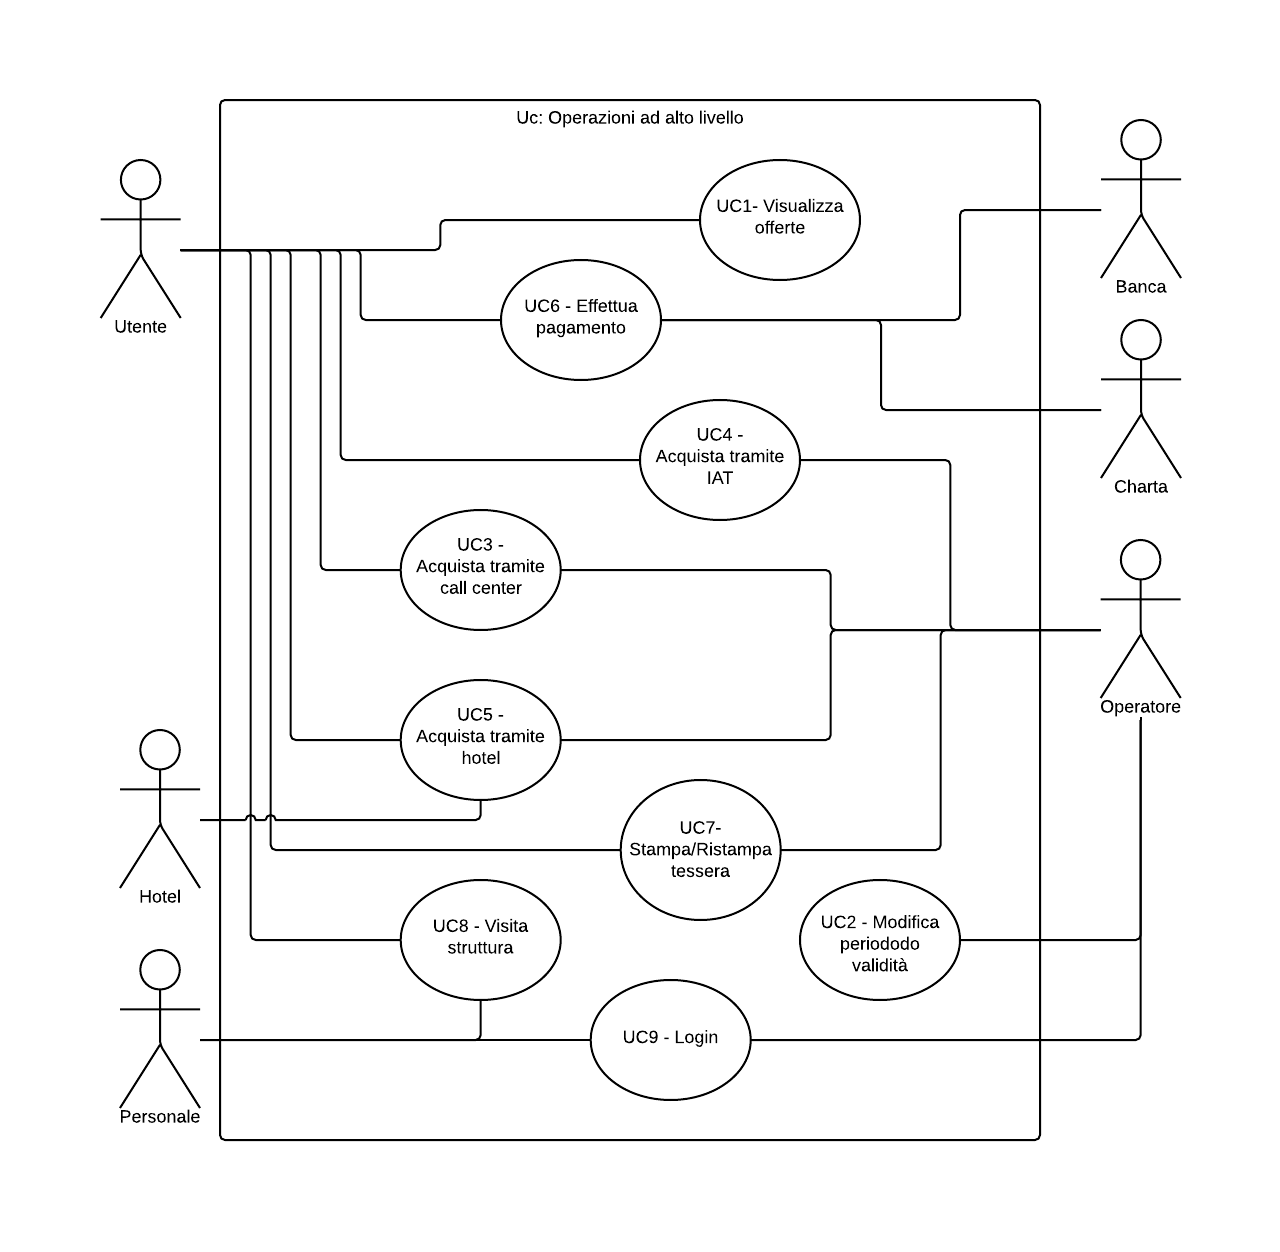
\includegraphics[width=1\textwidth]{images/UC.png}
\caption{Caso d'uso UC: Operazioni ad alto livello}
\end{figure}

\subsubsection{Caso d'uso UC1: Consultazione offerte}\label{UC1}
\begin{figure}[H]
\centering
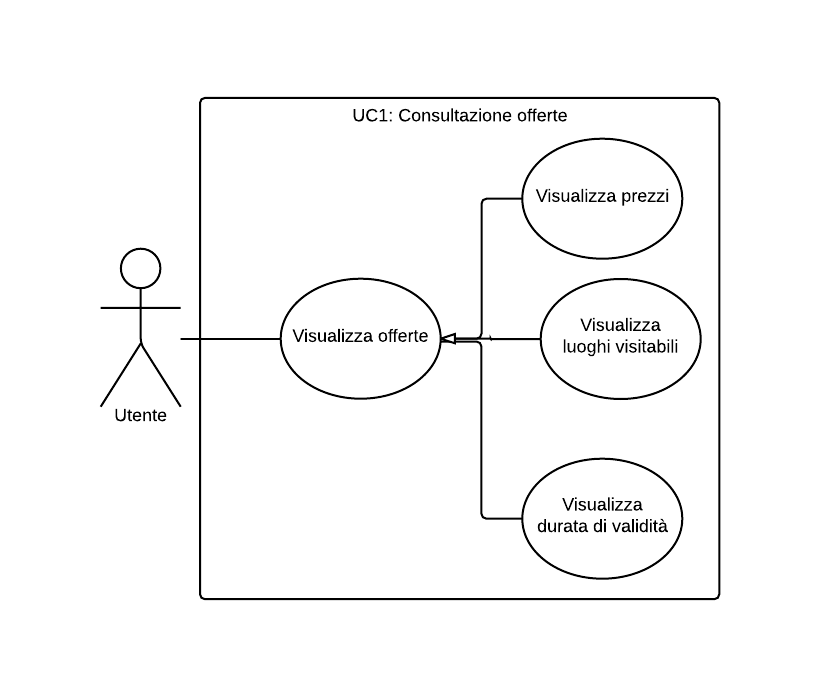
\includegraphics[width=1\textwidth]{images/UC1.png}
\caption{Caso d'uso UC1: Consultazione offerte}
\end{figure}
\begin{itemize}
\item \textbf{Attori:} Utente;
\item \textbf{Descrizione:} L'utente deve poter consultare online le offerte relative alla propria PadovaCard. Tali offerte comprendono i vari pacchetti con cui la PadovaCard viene proposta, i luoghi con essa visitabili ed i relativi costi e periodo di validità. Si tratta di un portale statico;

\item \textbf{Flusso principale degli eventi:}
	\begin{itemize}
		\item L'utente si collega al portale tramite browser;
		\item L'utente visualizza le informszioni a cui è interessato.
	\end{itemize}
\end{itemize}


\subsubsection{Caso d'uso UC2: Acquisto via internet}
\begin{figure}[H]
\centering
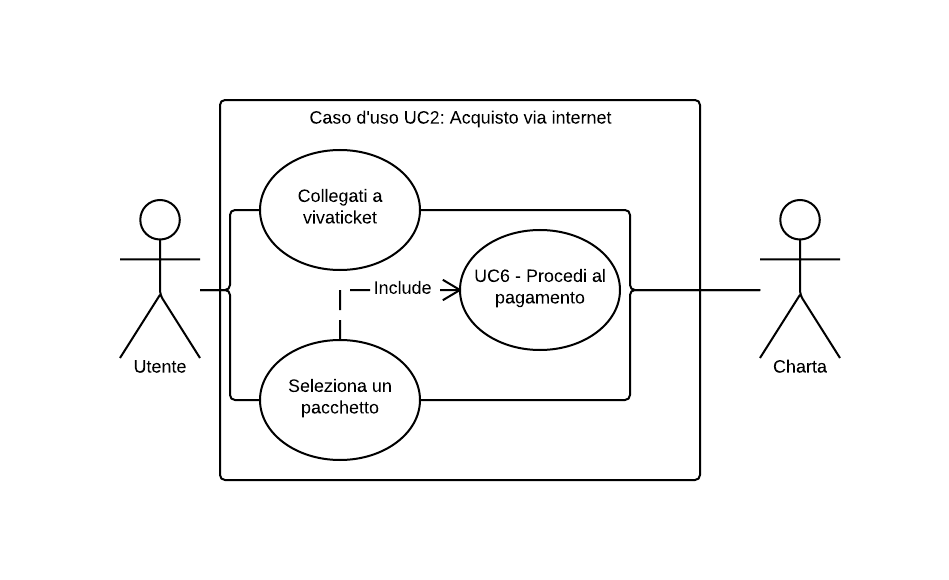
\includegraphics[width=1\textwidth]{images/UC2.png}
\caption{Caso d'uso UC2: Acquisto via internet}
\end{figure}
\begin{itemize}
\item \textbf{Attori:} Utente, \charta;
\item \textbf{Descrizione:} L'utente si collega alla piattaforma \vivaticket, direttamente o reinderizzato dal portale descritto in \ref{UC1}. Come già ora accade esso completerà l'operazione su \vivaticket. L'ultima operazione per poter ricevere le PadovaCard è il pagamento, descritto in \ref{UC6}.
\item \textbf{Precondizione:} L'utente desidera comprare una o più padova card;
\item \textbf{Flusso principale degli eventi:}
	\begin{itemize}
		\item L'utente si collega a \vivaticket;
		\item L'utente seleziona il pacchetto desiderato.
	\end{itemize}
\item \textbf{Postcondizione:}L'utente deve solamente pagare per completare l'acquisto.
\end{itemize}\subsubsection{PadovaCard ora}

\subsubsection{Caso d'uso UC3: Acquisto via call center}\label{UC3}
\begin{figure}[H]
\centering
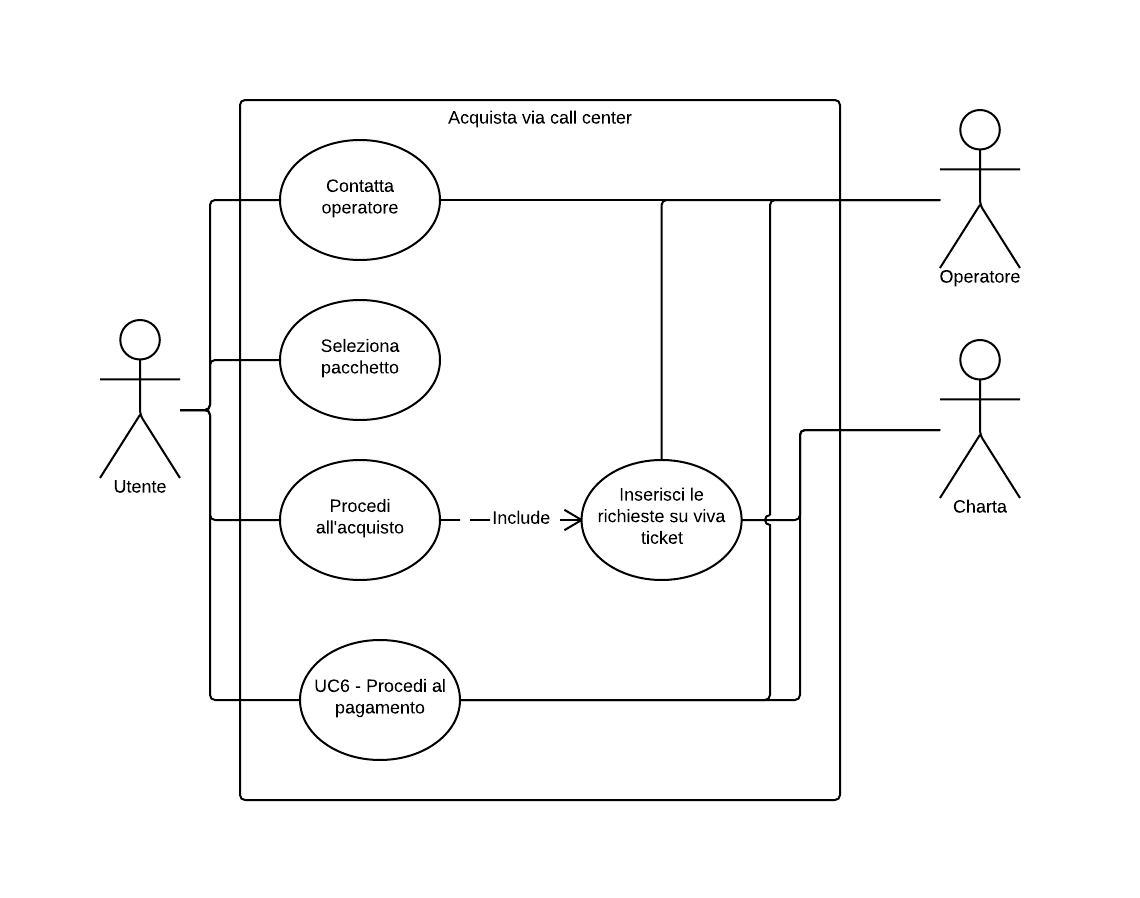
\includegraphics[width=1\textwidth]{images/UC3.png}
\caption{Caso d'uso UC3: Acquisto via call center}
\end{figure}
\begin{itemize}
\item \textbf{Attori:} Utente, operatore, \charta;
\item \textbf{Descrizione:} L'utente contatta il call center, e gli operatori guideranno l'utente nella scelta di uno dei pacchetti disponibili. Quando l'utente ha deciso l'operatore inserisce i dati su \tlite come già ora accade. L'ultima operazione per poter ricevere le PadovaCard è il pagamento, descritto in \ref{UC6}.
\item \textbf{Precondizione:} L'utente desidera comprare una o più padova card;
\item \textbf{Flusso principale degli eventi:}
	\begin{itemize}
		\item L'utente chiama il call center;
		\item L'utente, guidato dall'operatore sceglie quale pacchetto acquistare;
        \item L'operatore procede alla selezione su \tlite.
	\end{itemize}
\item \textbf{Postcondizione:}L'utente deve solamente pagare per completare l'acquisto.
\end{itemize}

\subsubsection{Caso d'uso UC4: Acquisto via IAT}\label{UC4}
\begin{figure}[H]
\centering
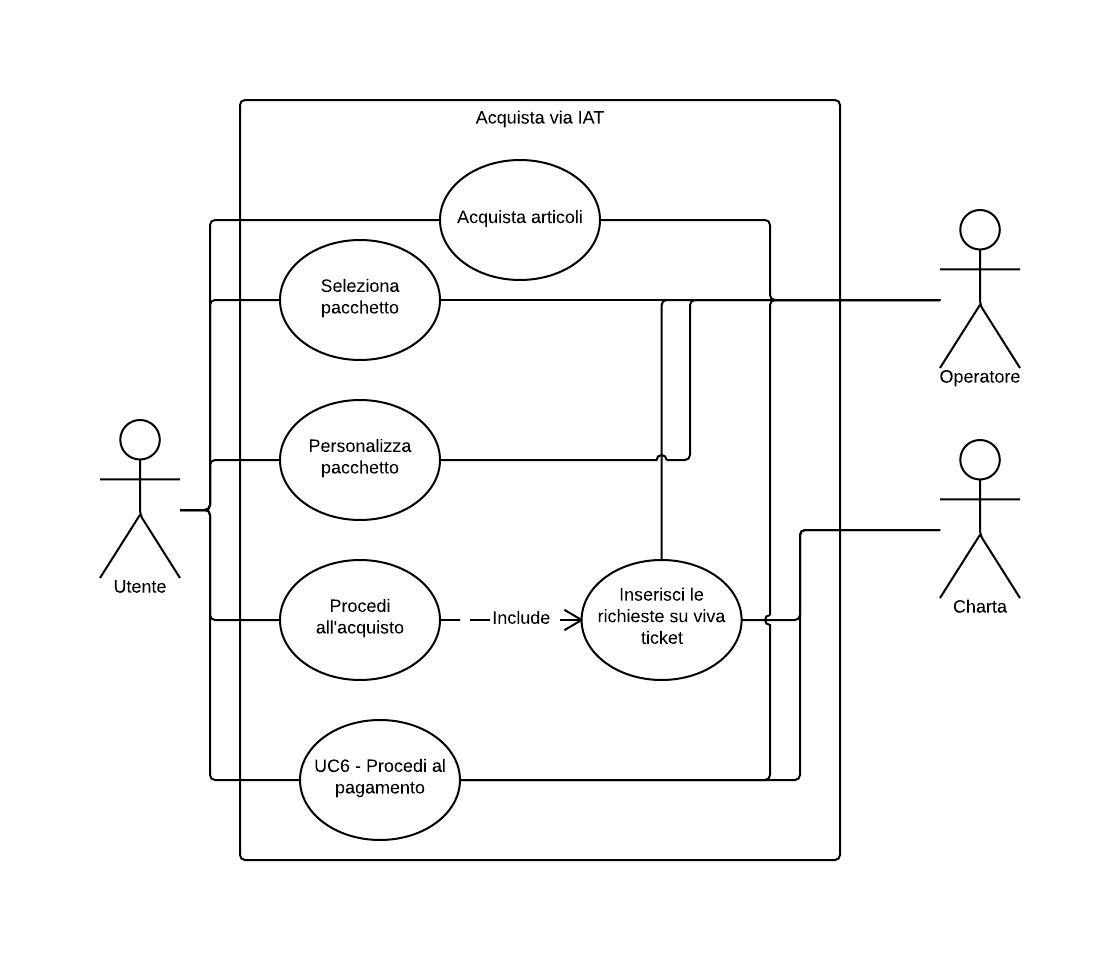
\includegraphics[width=1\textwidth]{images/UC4.png}
\caption{Caso d'uso UC4: Acquisto via IAT}
\end{figure}
\begin{itemize}
\item \textbf{Attori:} Utente, operatore, \charta;
\item \textbf{Descrizione:} L'utente si reca ad uno sportello IAT dove potrà acquistare uno degli articoli in vendita e/o una o più PadovaCard. L'operatore completerà la vendita su \tlite, ma in questo caso potrà poi personalizzare i pacchetti con le preferenze di visita e tempistiche dell'utente. A questo punto all'utente non resta che pagare quanto acquistato con un unico pagamento, tale operazione è illustrata nella Sezione \ref{UC6}.
\item \textbf{Precondizione:} L'utente desidera comprare una o più padova card;
\item \textbf{Flusso principale degli eventi:}
	\begin{itemize}
    	\item L'utente sceglie un pacchetto;
        \item L'operatore procede alla selezione su \tlite;
		\item L'utente assieme all'operatore personalizza il pacchetto;
		\item L'utente può acquistare altri articoli in vendita allo IAT.
	\end{itemize}
\item \textbf{Postcondizione:}L'utente deve solamente pagare per completare l'acquisto.
\end{itemize}

\subsubsection{Caso d'uso UC5: Acquisto via hotel}
\begin{figure}[H]
\centering
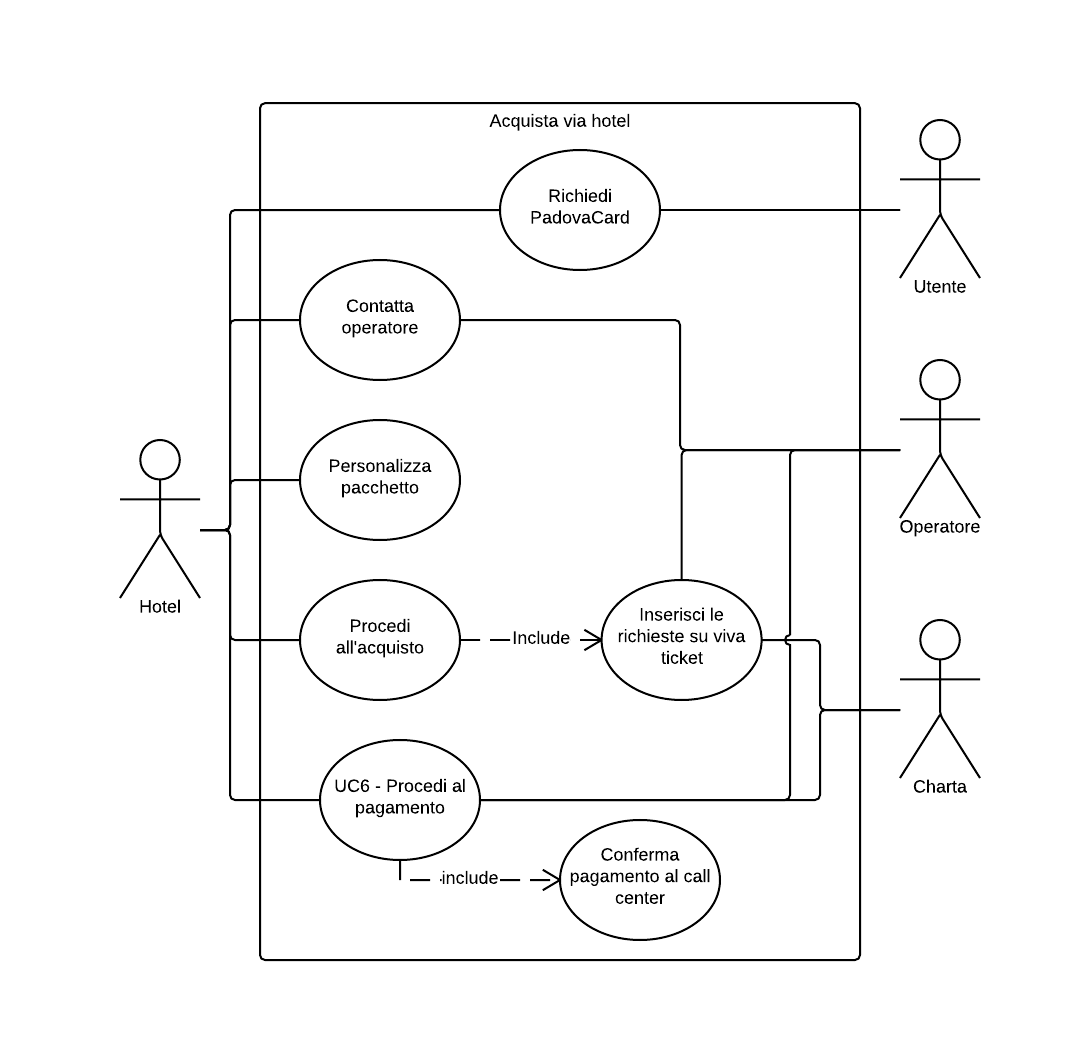
\includegraphics[width=1\textwidth]{images/UC5.png}
\caption{Caso d'uso UC5: Acquisto via hotel}
\end{figure}
\begin{itemize}
\item \textbf{Attori:} Utente, operatore, \charta, hotel;
\item \textbf{Descrizione:} L'utente riferisce ad un membro del personale dell'hotel (se quest'ultimo è convenzionato con PadovaCard) che desidera acquistare una o più PadovaCard. Il personale dell'hotel comunicherà con il call center, per i dettagli vedere il caso d'uso UC3 alla Sezione \ref{UC3}. Si tratterà però di una vendita speciale in quanto il pagamento non viene fatto su \tlite ma sulla piattaforma di PadovaCard. Quando l'operatore ha confermato la prenotazione si procederà alla personalizzazione della PadovaCard e al pagamento. Importante è che dopo l'avvenuto pagamento il call center viene notificato;
\item \textbf{Precondizione:} L'utente desidera comprare una o più padova card;
\item \textbf{Flusso principale degli eventi:}
	\begin{itemize}
    	\item L'utente riferisce all'hotel che desidera comprare una o più PadovaCard;
		\item L'hotel chiama il call center;
		\item L'hotel comunica quale pacchetto acquistare;
        \item L'operatore procede alla selezione su \tlite;
        \item L'hotel personalizza il pacchetto;
        \item Si procede al pagamento, e quando questo è avvenuto si notifica il call center, che conferma la prenotazione.
	\end{itemize}
\item \textbf{Postcondizione:}L'utente deve solamente pagare per completare l'acquisto;
\end{itemize}

\subsubsection{Caso d'uso UC6: Pagamento}\label{UC6}
\begin{figure}[H]
\centering
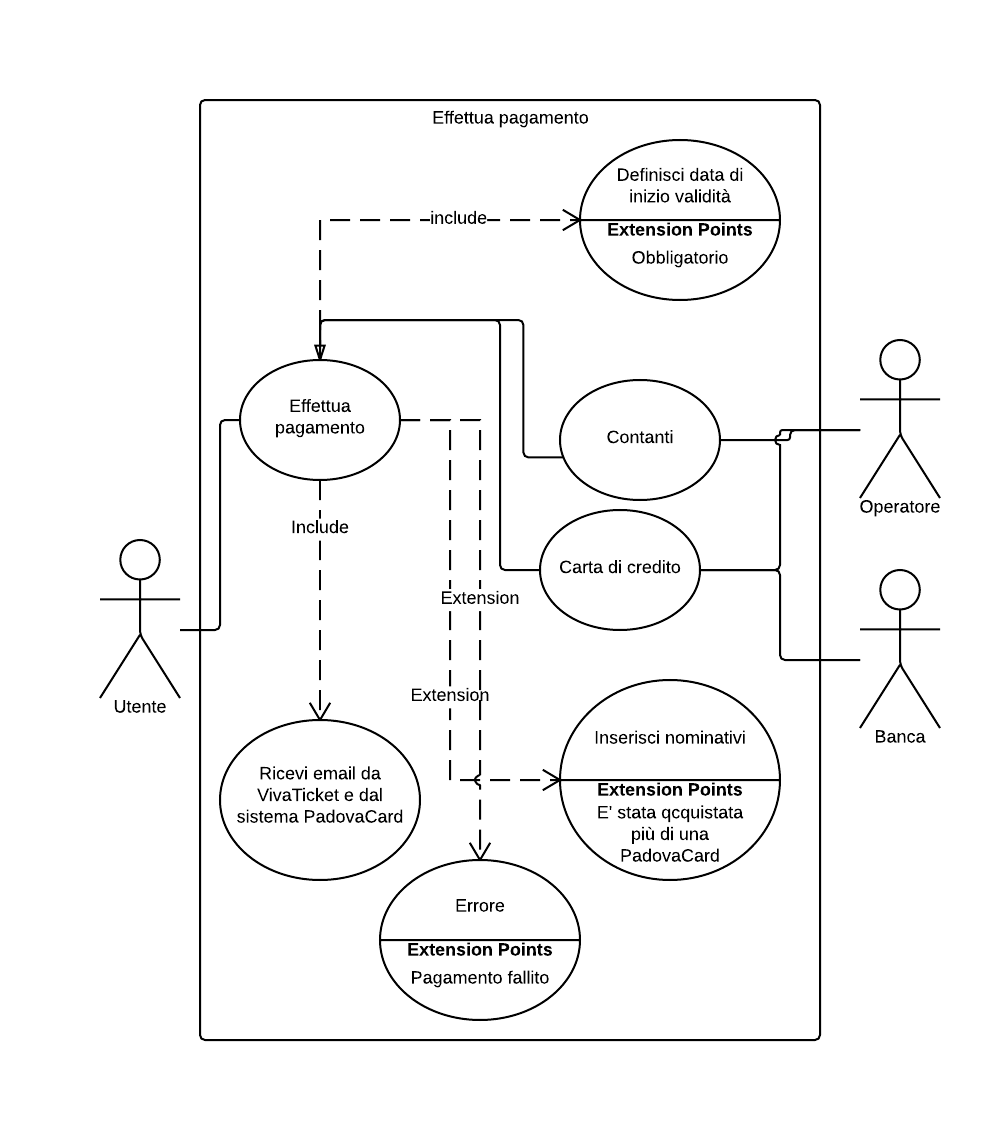
\includegraphics[width=1\textwidth]{images/UC6.png}
\caption{Caso d'uso UC6: Pagamento}
\end{figure}
\begin{itemize}
\item \textbf{Attori:} Utente, operatore, banca;
\item \textbf{Descrizione:} L'utente ha selezionato la propria PadovaCard con uno dei possibili metodi, e si appresta a pagare. E' possibile farlo sempre tramite carta di credito, mentre è possibile  in contanti solo se l'acquisto è stato fatto presso uno sportello IAT\textsuperscript{1}. Qualora il pagamento andasse a buon fine l'utente riceverà due email, una da \tlite     -\vivaticket, una dal sistema con il codice della PadovaCard. Qualora durante un'ordine siano acquistate più PadovaCard sarà necessario inserire un nominativo per ognuna di esse, avvalendosi di un operatore. Nel caso in cui l'acquisto avvenga via internet ciò non è possibile, ma una possibile soluzione è proposta come requisito facoltativo alla Sezione \ref{UCF3}.
Fondamentale è poi definire una data e un ora di inizio validità per la PadovaCard (la scadenza si fisserà di conseguenza), tenendo presente che se compresa, la visita alla cappella degli Scrovegni deve essere all'interno del periodo di validità.\\
\begin{footnotesize}
\textit{\textsuperscript{1} Un hotel a sua discrezione potrebbe far pagare l'utente in contanti e poi utilizzare la propria carta di credito}
\end{footnotesize}
\item \textbf{Precondizione:} L'utente ha selezionato il pacchetto da acquistare;
\item \textbf{Flusso principale degli eventi:}
	\begin{itemize}
		\item L'utente paga, via carta di credito o contanti;
        \item L'utente stabilisce la data e l'ora di inizio del periodo di validità;
		\item L'utente riceve la mail contenente il codice della PadovaCard.
	\end{itemize}
    \item \textbf{Flusso alternativo degli eventi:}
	\begin{itemize}
    	\item Il pagamento non va a buon fine, la carta è rifiutata dalla banca o l'utente non ha abbastanza contanti;
		\item L'utente acquista più di una PadovaCard, è necessario inserire i nominativi per ognuna.
	\end{itemize}
\item \textbf{Postcondizione:} L'utente ha ricevuto la PadovaCard.
\end{itemize}

\subsubsection{Caso d'uso UC7: Stampa/ristampa tessera}
\begin{figure}[H]
\centering
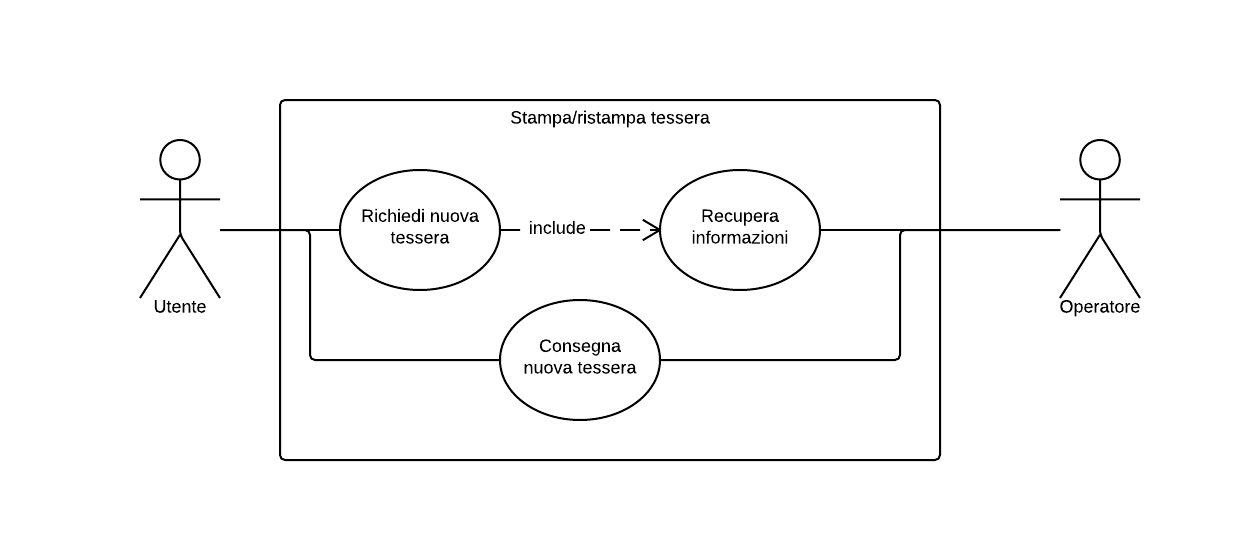
\includegraphics[width=1\textwidth]{images/UC7.png}
\caption{Caso d'uso UC7: Stampa/ristampa tessera}
\end{figure}
\begin{itemize}
\item \textbf{Attori:} Utente, operatore;
\item \textbf{Descrizione:}L'utente si reca ad uno sportello IAT e comunica la propria volontà di avere la propria PadovaCard stampata. Ricordiamo che avere la PadovaCard stampata non è strettamente necessario, in quanto è sufficiente stampare il codice ricevuto via email su carta o mostrare il codice a schermo. L'operatore recupera il codice della PadovaCard partendo dal nominativo dell'utente ed esegue la stampa;
\item \textbf{Precondizione:}L'utente desidera avere stampata la propria PadovaCard, o ha smarrito quella in suo possesso;
\item \textbf{Flusso principale degli eventi:}
	\begin{itemize}
    	\item L'utente desidera la PadovaCard stampata;
        \item L'operatore recupera il codice della PadovaCard;
        \item L'operatore stampa la PadovaCard.
    \end{itemize}
\item \textbf{Postcondizione:}  L'utente ottiene la PadovaCard stampata;
\end{itemize}

\subsubsection{Caso d'uso UC8: Visita struttura}
\begin{figure}[H]
\centering
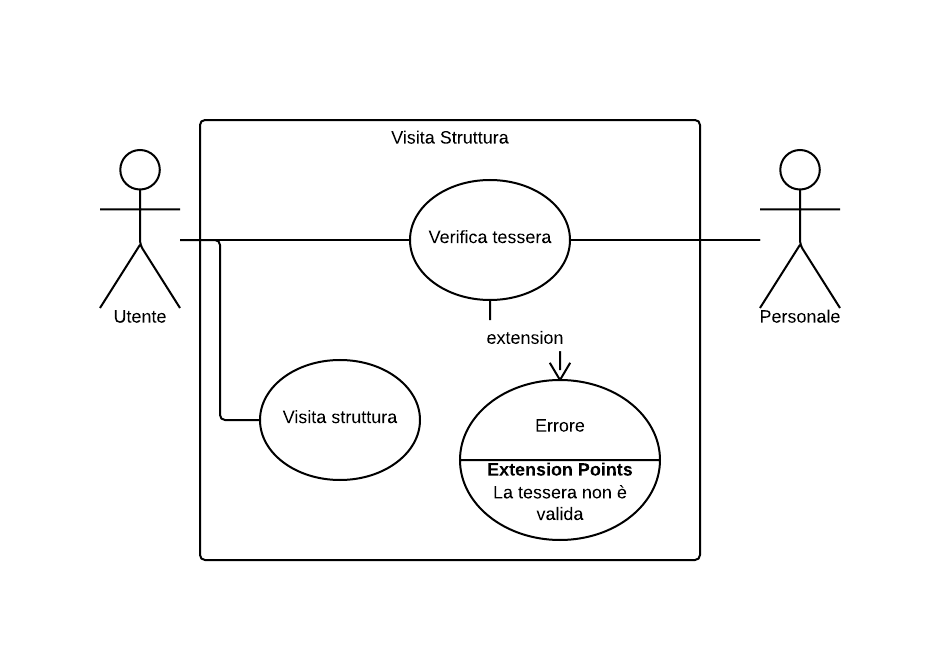
\includegraphics[width=1\textwidth]{images/UC8.png}
\caption{Caso d'uso UC8: Visita struttura}
\end{figure}
\begin{itemize}
\item \textbf{Attori:} Utente, personale;
\item \textbf{Descrizione:} Un utente munito della propria PadovaCard si reca alla struttura che desidera visitare, il personale, autenticato nel sistema legge il codice a barre (stampato o a schermo) tramite l'apposito lettore e visualizza quindi sul monitor se l'utente può visitare la struttura o meno;
\item \textbf{Precondizione:} L'utente vuole visitare una struttura, il personale è autenticato;
\item \textbf{Postcondizione:}  L'utente ha visitato la struttura;
\end{itemize}


\subsubsection{Caso d'uso UC9: Login}
\begin{figure}[H]
\centering
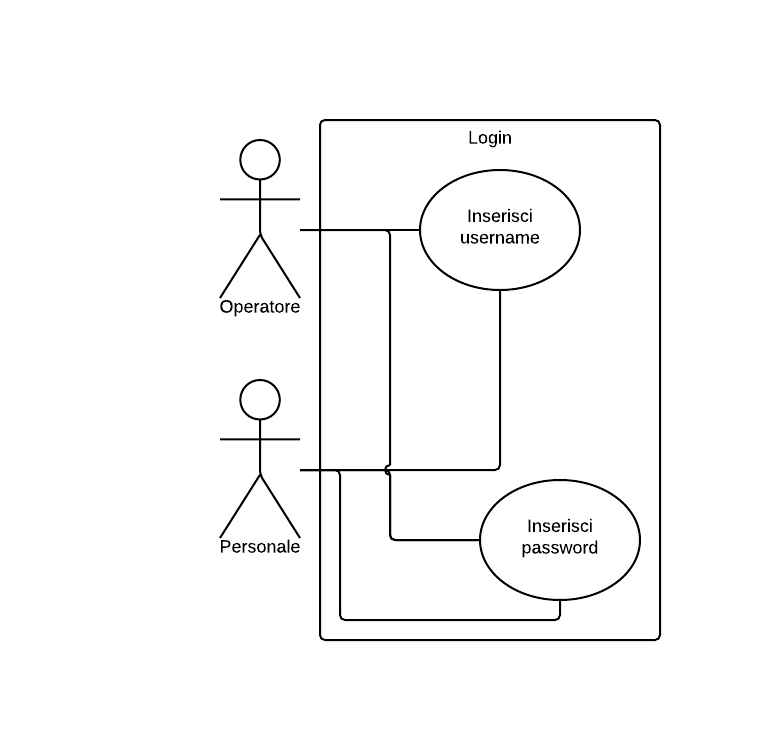
\includegraphics[width=1\textwidth]{images/UC9.png}
\caption{Caso d'uso UC9: Login}
\end{figure}
\begin{itemize}
\item \textbf{Attori:} Personale, operatore;
\item \textbf{Descrizione:} Vengono inserite le credenziali, username e password e se corretti si viene autenticati;
\item \textbf{Precondizione:} Il personale e gli operatori non sono autenticati;
\item \textbf{Postcondizione:}  Il personale e gli operatori sono autenticati.
\end{itemize}

\subsubsection{Caso d'uso UC10: Modifica periodo validità}
\begin{figure}[H]
\centering
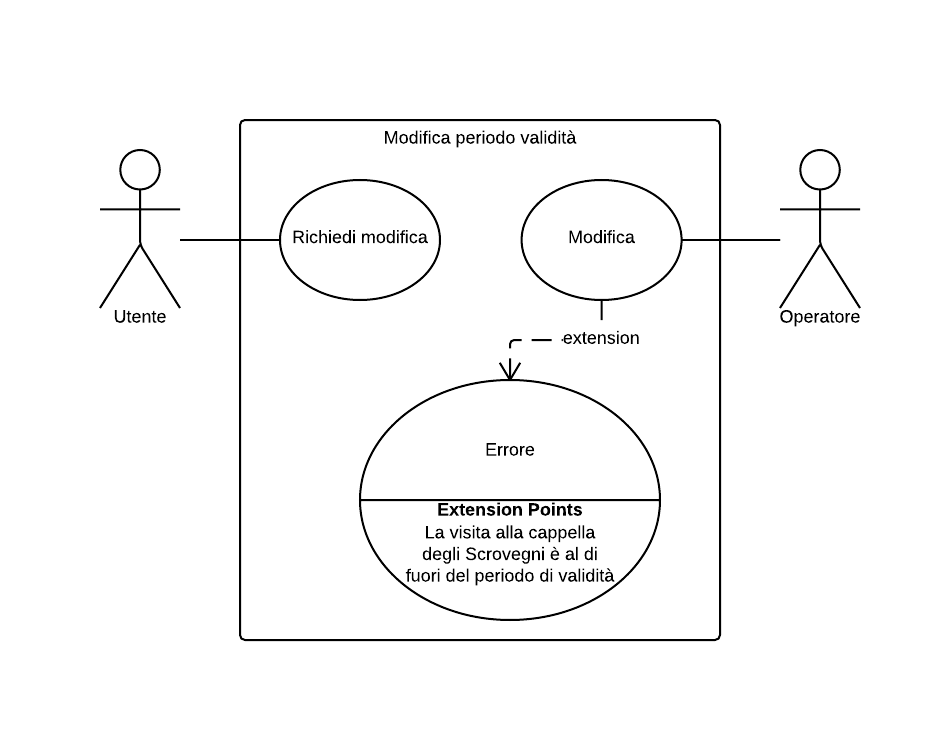
\includegraphics[width=1\textwidth]{images/UC10.png}
\caption{Caso d'uso UC10: Modifica periodo validità}
\end{figure}
\begin{itemize}
\item \textbf{Attori:} Utente, operatore;
\item \textbf{Descrizione:} L'utente ha acquistato una o più PadovaCard, e nel momento dell'acquisto ha definito il loro periodo di validità, selezionando data e ora, come descritto in UC6, alla Sezione \ref{UC6}. L'utente decide però di modificare tale periodo di validità, non gli è consentito farlo da solo, dovrà quindi contattare un operatore, call center o IAT e far modificare il peridoo di validità, con il vincolo che se è prevista una visita alla cappella degli Scrovegni, essa non può essere spostata, per cui tale visita dovrà trovarsi sempre dentro l'arco temporale di validità della tessera;
\item \textbf{Precondizione:} L'utente desidera modificare il periodo di validità della PadovaCard;
\item \textbf{Postcondizione:}  Il periodo di validità della PadovaCard è modificato.
\end{itemize}

\subsubsection{Caso d'uso UCF: Operazioni ad alto livello}\label{UCF}
Il seguente diagramma mostra una visione ad alto livello dei casi d'uso facoltativi. Ogni caso d'uso è analizzato nel dettaglio nelle sezioni successive. I casi d'uso obbligatori si trovano dalla Sezione \ref{UC} in poi.
\begin{figure}[H]
\centering
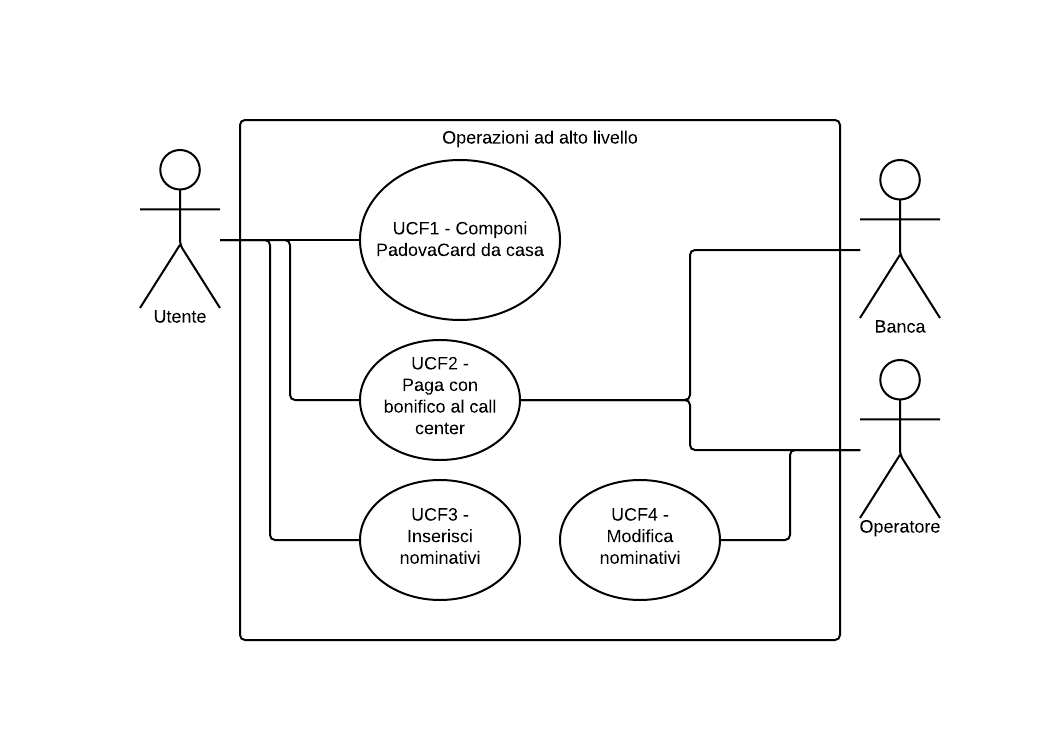
\includegraphics[width=1\textwidth]{images/UCF.png}
\caption{Caso d'uso UCF: Operazioni ad alto livello}
\end{figure}

\subsubsection{Caso d'uso UCF1: Componi PadovaCard da casa}
Questo requisito permette all'utente di personalizzare la propria PadovaCard da casa.
\begin{figure}[H]
\centering
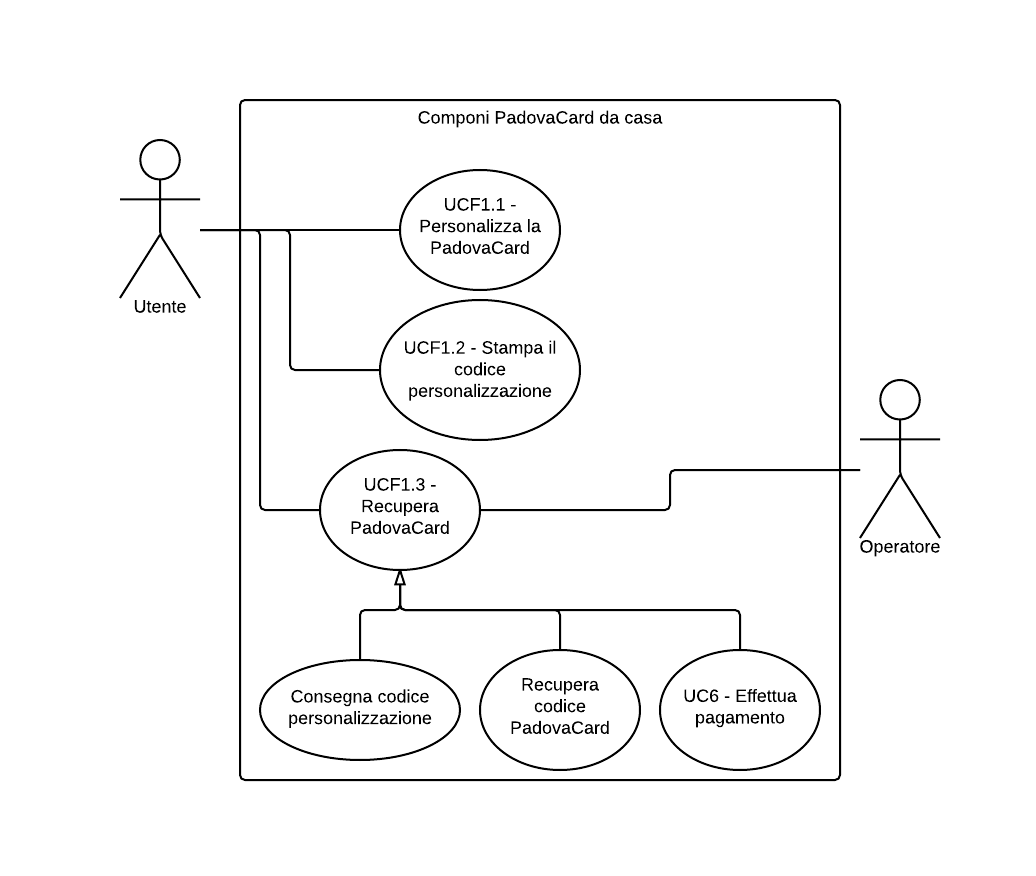
\includegraphics[width=1\textwidth]{images/UCF1.png}
\caption{Caso d'uso UCF1:  Componi PadovaCard da casa}
\end{figure}
\textbf{UCF1.1}
\begin{itemize}
\item \textbf{Attori:} Utente;
\item \textbf{Precondizione:} L'utente accede al portale;
\item \textbf{Descrizione:} L'utente tramite il portale web ha la possibilità di comporre la propria Padovacard;
\item \textbf{Postcondizione:} L'utente ha personalizzato la propria PadovaCard.
\end{itemize}

\textbf{UCF1.2}
\begin{itemize}
\item \textbf{Attori:} Utente;
\item \textbf{Precondizione:} L'utente ha personalizzato la propria PadovaCard;
\item \textbf{Descrizione:} Il portale genera un codice di personalizzazione. Tale codice non è da confondere con quello della PadovaCard, esso infatti non permette di accedere alle strutture;
\item \textbf{Postcondizione:} L'utente è in possesso di un codice di personalizzazione.
\end{itemize}

\textbf{UCF1.3}
\begin{itemize}
\item \textbf{Attori:} Utente, operatore;
\item \textbf{Precondizione:} L'utente è in possesso di un codice di personalizzazione;
\item \textbf{Descrizione:} L'utente con il proprio codice di personalizzazione si reca ad uno sportello IAT, dove l'operatore, leggendo il codice ed interrogando il sistema verrà a conoscenza di come l'utente desidera la propria PadovaCard. Questo sistema permette di velocizzare la creazione della PadovaCard. Da questo momento in poi il procedimento è lo stesso di UC4, visibile alla Sezione \ref{UC4}.

\item \textbf{Postcondizione:} L'utente è in possesso della PadovaCard.
\end{itemize}

\subsubsection{Caso d'uso UCF2: Pagamento con bonifico}
\begin{figure}[H]
\centering
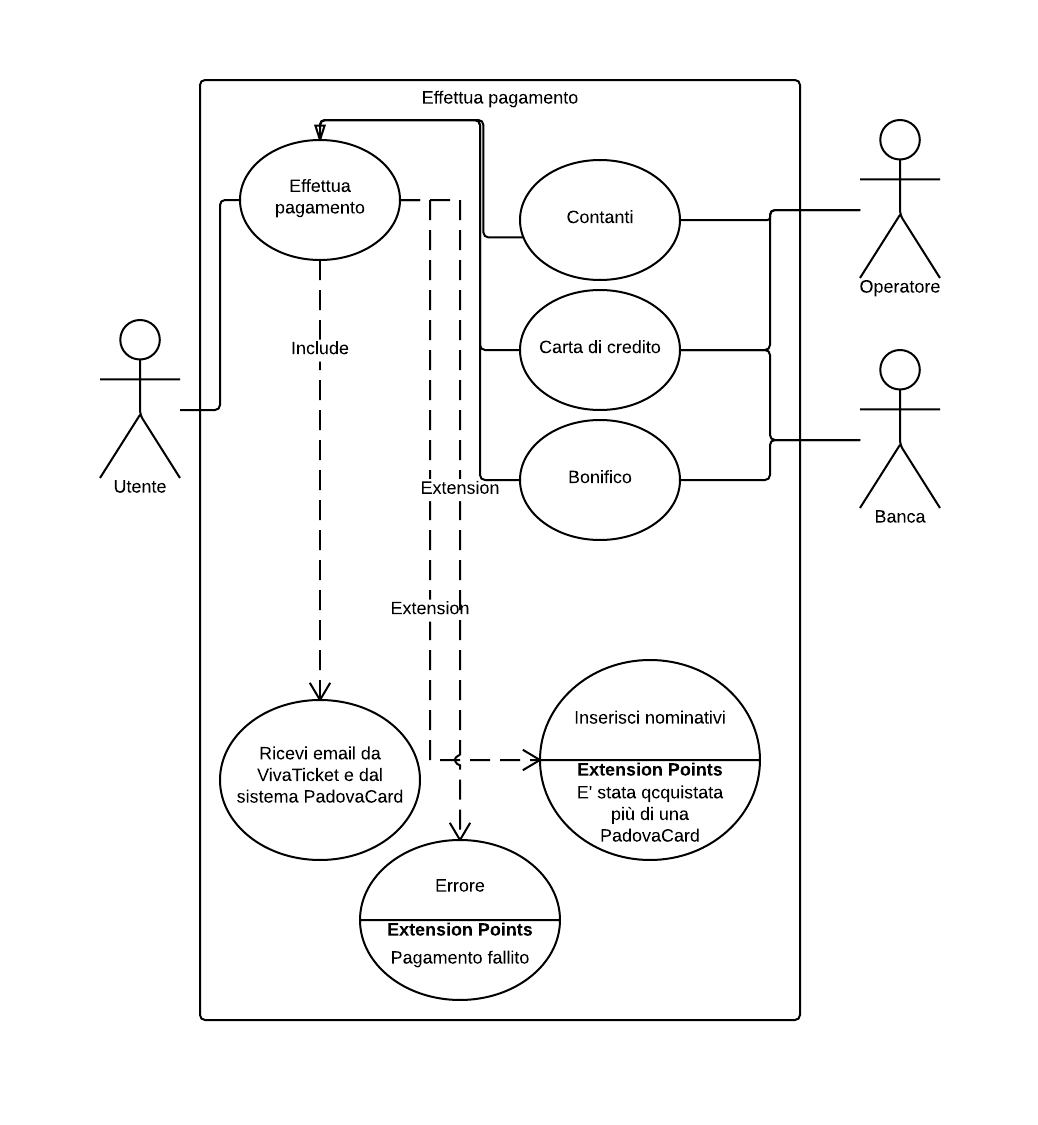
\includegraphics[width=1\textwidth]{images/UCF2.png}
\caption{Caso d'uso UCF2: Pagamento con bonifico}
\end{figure}
\begin{itemize}
\item \textbf{Attori:} Utente, operatore, banca;
\item \textbf{Descrizione:} Si tratta del caso d'uso UC6, consultabile alla Sezione \ref{UC6}, con l'aggiunta della possibilità per l'utente di pagare tramite bonifico bancario. In questa eventualità l'operatore effettuerà la prenotazione su \tlite, ma attenderà la conferma del bonifico da parte della banca prima di procedere alla conferma della prenotazione, che scatenerà tutti i successivi eventi (ricezione email, generazione codice Padovacard etc.);
\item \textbf{Precondizione:} L'utente ha selezionato il pacchetto da acquistare;
\item \textbf{Postcondizione:}  L'utente ha ricevuto la PadovaCard.
\end{itemize}


\subsubsection{Caso d'uso UCF3: Inserisci nominativi}\label{UCF3}

\begin{figure}[H]
\centering
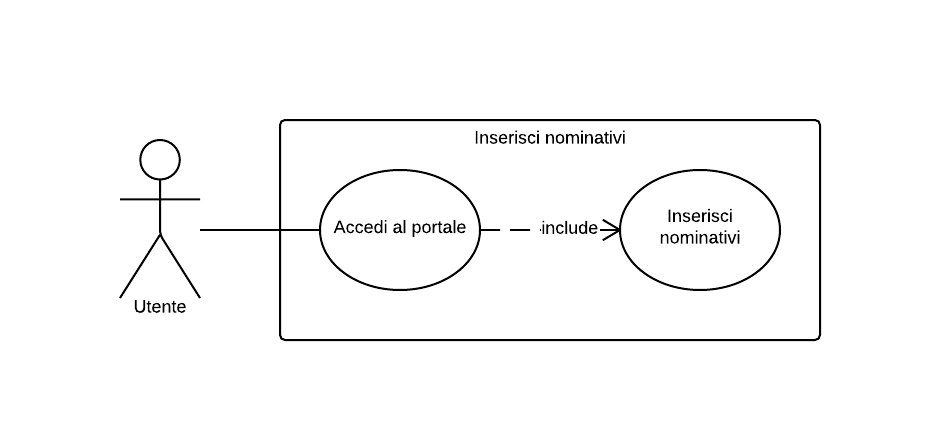
\includegraphics[width=1\textwidth]{images/UCF3.png}
\caption{Caso d'uso UCF3: Inserisci nominativi}
\end{figure}
\begin{itemize}
\item \textbf{Attori:} Utente;
\item \textbf{Descrizione:} Di fronte ad un ordine di più PadovaCard si pone il problema dei nominativi ad esse correlati, come descritto in UC6 - Pagamento (Sezione \ref{UC6}). Per ovviare al problema nel caso in cui l'utente abbia effettuato l'ordine via internet è possibile rendere disponibile una funzionalità che permette all'utente stesso di inserire i nominativi, accedendo al sistema con il codice dell'ordine effettuato su \vivaticket e compilando i form che gli vengono presentati.
\item \textbf{Precondizione:} L'utente è in possesso di più PadovaCard;
\item \textbf{Postcondizione:}  L'utente ha collegato un nominativo per ogni PadovaCard in suo possesso.
\end{itemize}

\subsubsection{Caso d'uso UCF4: Modifica nominativi}
Non è presente un diagramma UML in quanto si tratta di un caso d'uso semplicissimo.
\begin{itemize}
\item \textbf{Attori:} Operatore;
\item \textbf{Descrizione:} Assumendo che l'utente abbia inserito i nominativi, come descritto in UCF3, Sezione \ref{UCF3}, deve essere possibile modificarli, in caso di errore. Se si da tale possibilità all'utente c'è il rischio che ne approfitti per associare diversi proprietari ad un unica PadovaCard, anche se non contemporaneamente. 
L'utente che vuole modificare tali nominativi dovrà quindi contattare un operatore e richiedere la modifica.
\item \textbf{Precondizione:} L'utente ha inserito i nominativi per ogni Padovacard del suo ordine;
\item \textbf{Postcondizione:} L'operatore ha modificato uno o più nominativi.
\end{itemize}

\subsection{Requisiti}
Ogni requisito è identificato da un codice, che segue il seguente formalismo:

\begin{center}
\textbf{R\{X\}\{Y\} \{Gerarchia\}}
\end{center}

Dove:
\begin{itemize}
\item X corrisponde alla priorità del requisito e può assumere i seguenti valori:
	\begin{itemize}
		\item O = Obbligatorio;
        \item F = Facoltativo o opzionale.
	\end{itemize}
\item Y corrisponde al sistema di riferimento e può assumere i seguenti valori:
	\begin{itemize}
		\item O = Operatore, si tratta di operatori degli sportelli IAT o del call center;
        \item U = Utente, si tratta del fruitore della PadovaCard, tipicamente un turista;
        \item P = Personale, si tratta del personale dei luoghi d'interesse convenzionati con PadovaCard;
        \item S = Sistema, si tratta del sistema che si occupa della gestione della PadovaCard.
	\end{itemize}
\item Gerarchia identifica la relazione gerarchica che c'è tra i requisiti di uno stesso tipo. C'è quindi una struttura gerarchica per ogni tipologia di requisito.
\end{itemize}

\newpage

\def\arraystretch{2}
\begin{center}
\begin{longtable}[H]{| p{.20\textwidth} | p{.60\textwidth} | p{.20\textwidth}|}
\hline 
Requisito & Descrizione & Fonti \\ \hline
ROU 1 & L'utente deve poter consultare online le offerte relative alla propria padova card  & UC1 \\ \hline
ROU 2 & L'utente può acquistare uno degli n pacchetti preconfigurati su \vivaticket pagando con carta di credito e ricevere via mail il codice. & UC2, UC6 \\ \hline
ROU 3 & L'utente, tramite operatore deve poter comunicare i nominativi associati ad ogni tessera, se su \tlite ne è stata acquistata più di una all'interno di un solo ordine. & UC6 \\ \hline
ROU 4 & L'utente può acquistare uno degli n pacchetti preconfigurati chiamando il call center, pagando con carta di credito e ricevere via mail il codice. & UC3, UC6 \\ \hline
ROU 5 & L'utente può acquistare uno degli n pacchetti preconfigurati in uno degli alberghi convenzionati pagando con carta di credito o contanti e riceve via mail il codice, e opzionalmente un \glossario{voucher}. & UC5, UC6 \\ \hline
ROU 6 & L'utente può acquistare uno degli n pacchetti preconfigurati, o comporre il proprio ad uno sportello IAT, pagando con carta di credito o contanti e riceverà la tessera e via mail il codice.  & UC4, UC6 \\ \hline
ROU 7 & L'utente può accedere alla struttura solo se è prevista all'interno della sua padovacard, se essa non è scaduta (superato il periodo di validità) e se non ha già effettuato la visita.  & UC8 \\ \hline
ROU 8 & L'utente può farsi stampare una nuova tessera in caso essa venga smarrita. (L'utente è comunque in possesso del codice su email).  & UC7 \\ \hline
ROU 9 & L'utente deve inserire la data e l'ora di inizio validità della PadovaCard.  & UC6 \\ \hline
RFU 10 & L'utente può comporre la propria padova card, visualizzando in tempo reale prezzi ed offerte dei vari pacchetti/ingressi.  & UCF1.1, UCF1.2, UCF1.3 \\ \hline
RFU 11 & L'utente può stampare un codice relativo alla propria composizione ed acquistarla ad uno sportllo IAT.  & UCF1.2, UCF1.3 \\ \hline
RFU 12 & L'utente può acquistare uno degli n pacchetti preconfigurati chiamando il call center, pagando con bonifico e ricevere via mail il codice.   & UCF2 \\ \hline
RFU 13 & L'utente, tramite il portale deve poter inserire i nominativi associati ad ogni tessera, se su vivaticket ne è stata acquistata più di una all'interno di un solo ordine.  & UCF3 \\ \hline
ROP 14 & Il personale deve loggarsi al sistema con un id univoca.  & UC9 \\ \hline
ROP 15 & Il personale avrà un lettore di codici che rileverà il codice presente sulla tessera, sul \glossario{voucher} o a a schermo, nel caso in cui l'utente utilizzi la mail su cellulare.  & UC8 \\ \hline
ROO 16 & Gli operatori devono loggarsi al sistema con un id univoca.  & UC9 \\ \hline
ROO 17 & Gli operatori potranno selezionare uno degli n pacchetti preconfigurati su \tlite  & UC4, UC3 \\ \hline
ROO 18 & L'operatore dovrà poter inserire nel sistema i nominativi associati alle padovacard se queste sono state acquistate su \tlite tramite un unico ordine.  & UC6 \\ \hline
ROO 19 & Gli operatori IAT di effettuare un unico pagamento nel caso in cui vengano combinati l'acquisto di una o più padova card sia con i pacchetti predefiniti sia personalizzate e altri articoli in vendita (mappe, guide, souvenir etc.). & UC6 \\ \hline
ROO 20 & Gli operatori possono modificare, su richiesta dell'utente il periodo di validità di una Padovacard già acquistata. & UC10 \\ \hline
ROS 21 & Il sistema riceverà i dati da \tlite e li inserirà nel database, salvando la vendita, per ragioni amministrative.  &  \\ \hline
ROS 22 & Il sistema partendo dai dati ricevuti da \tlite genererà un codice univoco per ogni tessera e vi associerà tutte le informazioni, per poi salvarle nel database.  &  \\ \hline
ROS 23 & Allo scadere del periodo di validità il sistema marca il codice della carta come non più valida. &  \\ \hline
ROS 24 & Quando si effettua una visitail sistema marca tale visita non più effettuabile da parte di quel codice.  &  \\ \hline
ROS 25 & Il sistema mantiene separati I dati relativi alle PadovaCard da tutti gli altri, ma raggruppa I dati sulle vendite, per cui la vendita di una PadovaCard è salvata assieme a qualunque altra vendita, ma nessuna informazione è fornita su tale padovaCard se non il codice.  &  \\ \hline
RFS 26 & Il sistema ricnosce come non valida una tessera a cui non è associato un nominativo &  \\ \hline
RFS 27 & Il sistema permette di associare un nominativo ad una carta dal momento in cui essa è creata a quello in cui perde la sua validità. &  \\ \hline
RFS 27 & Il sistema non permette ad un utente di modificare il nominativo associato ad una carta, lo permette invece ad un operatore.   &  \\ \hline

\caption{Tabella requisiti}
\end{longtable}
\end{center}

